\documentclass{article}
\usepackage{epsfig,placeins}

%
% Copyright (C) 2007 Alan D. Brunelle <Alan.Brunelle@hp.com>
%
%  This program is free software; you can redistribute it and/or modify
%  it under the terms of the GNU General Public License as published by
%  the Free Software Foundation; either version 2 of the License, or
%  (at your option) any later version.
%
%  This program is distributed in the hope that it will be useful,
%  but WITHOUT ANY WARRANTY; without even the implied warranty of
%  MERCHANTABILITY or FITNESS FOR A PARTICULAR PURPOSE.  See the
%  GNU General Public License for more details.
%
%  You should have received a copy of the GNU General Public License
%  along with this program; if not, write to the Free Software
%  Foundation, Inc., 59 Temple Place, Suite 330, Boston, MA  02111-1307  USA
%
%  vi :set textwidth=75

\title{\texttt{btt} User Guide}
\author{Alan D. Brunelle (Alan.Brunelle@hp.com)}
\date{10 April 2007}

\begin{document}
\maketitle
%--------------
\section{\label{sec:intro}Introduction}

\texttt{btt} is a post-processing tool for the block layer IO tracing tool called blktrace. As noted in its Users Guide, blktrace 
  \begin{quotation}
    is a block layer IO tracing mechanism which provides detailed
    information about request queue operations up to user space.
  \end{quotation}

blktrace is capable of producing tremendous amounts of output in the
form of multiple individual traces per IO executed during the traced
run. It is also capable of producing some general statistics concerning
IO rates and the like. \texttt{btt} goes further and produces a variety
of overall statistics about each of the individual handling of IOs, and
provides data we believe is useful to plot to provide visual comparisons
for evaluation.

This document will discuss \texttt{btt} usage, provide some sample output,
and also show some interesting plots generated from the data provided
by the \texttt{btt} utility.

\bigskip
A short note on the ordering of this document -- the actual
command-line usage section occurs relatively late in the document (see
section~\ref{sec:cmd-line}), as we felt that discussing some of the
capabilities and output formats would make the parameter discussion
easier.

\bigskip
  This document refers to the output formats generated by \texttt{btt}
  version 0.99.1.  However, the descriptions are general enough to cover
  output formats prior to that.

\newpage\tableofcontents

\newpage\section{\label{sec:getting-started}Getting Started}

  The simple pipeline to get going with \texttt{btt} is to perform the
  following steps:

  \begin{enumerate}
    \item Run \texttt{blktrace}, specifying whatever devices and other
    parameters you want. You must save the traces to disk in this step,
    btt does not work in live mode.

    \item After tracing completes, run \texttt{blkrawverify}, specifying
    all devices that were traced (or at least on all devices that you
    will use \texttt{btt} with -- section~\ref{sec:o-D} shows how you
    can dictate which devices to use with btt). If blkrawverify finds
    errors in the trace streams saved, it is best to recapture the data
    -- utilizing \texttt{btt} on \emph{unclean} trace files produces
    inconsistent results.

    While this step is optional, we have found that performing this
    helps to ensure data coming from \texttt{btt} makes the most sense.

    \item Run \texttt{blkparse} with the \texttt{-d} option specifying
    a file to store the combined binary stream. (e.g.: \texttt{blkparse
    -d bp.bin ...}).

    \texttt{blktrace} produces a series of binary files
    containing parallel trace streams -- one file per CPU per
    device. \texttt{blkparse} provides the ability to combine all the
    files into one time-ordered stream of traces for all devices.

    \item Run \texttt{btt} specifying the file produced by
    \texttt{blkparse} utilizing the \texttt{-i} option (e.g.: \texttt{btt
    -i bp.bin ...}).

  \end{enumerate}

\newpage\section{\label{sec:output-overview}Output Overview}

  The major default areas of output provided by \texttt{btt}
  include\label{tl-defs}:

\begin{description}
  \item[average component times across all IOs] The time line of each IO
  is broken down into 3 major regions:

    \begin{enumerate}
      \item Time needed to insert or merge an incoming IO onto the request
      queue. This is the average time from when the IO enters the block
      IO layer (queue trace) until it is inserted (insert trace) or merged
      (back merge or front merge trace).

      This is denoted as \emph{Q2I} time.

      \item Time spent on the request queue. The average time from when
      the IO is inserted or merged onto the request queue, until it is
      issued (issue trace) to the lower level driver.

      Referred to as \emph{I2D} time\footnote{The \emph{issue} trace
      is represented by a D in the blkparse output, hence its usage in
      btt to refer to issue traces. Note that an I is used to refer to
      \emph{insert} traces.}.

      \item Driver and device time -- the average time from when the
      actual IO was issued to the driver until is completed (completion
      trace) back to the block IO layer.

      This is referred to as the \emph{D2C} time\
    \end{enumerate}

  Two other sets of results are presented in this section:

    \begin{enumerate}
      \item \emph{Q2Q} which measures the time between queue traces
      in the system. This provides some idea as to how quickly IOs are
      being handed to the block IO layer.

      \item \emph{Q2C} which measures the times for the complete life cycle
      of IOs during the run\footnote{One of the areas that needs some
      work in \texttt{btt} is to better understand the multiplex nature of
      IOs during a run. In theory, one would like ${Q2I} + {I2D} + {D2C}
      = {Q2C}$ however, typically there are multiple queue traces that
      are combined via merges into a single IO issued and completed. We
      currently average the queue-to-insert and queue-to-merge times,
      and thus tend to be quite close to the expected equation.}

    \end{enumerate}

  For each row in this output, we provide a minimum, average, maximum
  (which are all presented in seconds), and overall count. As an
  example\footnote{As with this display, the author has taken some liberty
  in reformatting the output for better display on the printed page.}:

\begin{verbatim}
ALL            MIN           AVG           MAX           N
---- ------------- ------------- ------------- -----------
Q2Q    0.000000058   0.000012761   9.547941661     2262310
Q2I    0.000000272   0.000005995   0.104588839     2262311
I2D    0.000001446   0.094992714   0.239636864     2262311
D2C    0.000193721   0.030406554   1.634221408     2262311
Q2C    0.000207665   0.125405263   1.830917198     2262311
\end{verbatim}

  \item[Device Overhead]

  Using the data from the previous chart, we can then provide some idea
  as to where IO spend most of the time on average. The following output
  shows the percentage of time spent in each of the 3 phases of an IO:

\begin{verbatim}
       DEV |    Q2I    I2D    D2C
---------- | ------ ------ ------
 ( 68, 64) |   0.0%  75.7%  24.2%
\end{verbatim}

  \item[Device Merge Information]

  A key measurement when making changes in the system (software \emph{or}
  hardware) is to understand the block IO layer ends up merging incoming
  requests into fewer, but larger, IOs to the underlying driver. In this
  section, we show the number of incoming requests (Q), the number of
  issued requests (D) and the resultant ratio. We also provide values
  for the minimum, average and maximum IOs generated.

  Looking at the following example:

\begin{verbatim}
       DEV |      #Q    #D Ratio | BLKmin BLKavg BLKmax   Total
---------- | ------- ----- ----- | ------ ------ ------ -------
 ( 68, 64) | 2262311 18178 124.5 |      2    124    128 2262382
\end{verbatim}

  we see that (on average) the block IO layer is combining upwards of
  125 incoming requests into a single request down the IO stack. The
  resultant average IO size is 124 blocks.

  \item[Device Seek Information]

  Another useful measure is the variability in the sector distances
  between consecutive IOs. The next session provides some rudimentary
  statistics to gauge the general nature of the sector differences
  between IOs. Values provided include the number of seeks (number of IOs
  submitted to lower level drivers), the \emph{mean} distance between
  IOs, the \emph{median} value for all seeks, and the \emph{mode} -
  the value(s) and the counts are provided for the latter.

\begin{verbatim}
      DEV | NSEEKS    MEAN MEDIAN | MODE
--------- | ------ ------- ------ | -------
( 68, 64) |  18178 19611.3      0 | 0(17522)
\end{verbatim}

  We have almost exclusively seen median and mode values of 0, indicating
  that seeks tend to have an equal amount of forward and backwards
  seeks. The larger the count for the mode in comparison to the total
  number of seeks is indicative as to how many IOs are coming out of
  the block IO layer in adjacent sectors. (Obviously, the higher this
  percentage, the better the underlying subsystems can handle them.)


  \item[Request Queue Plug Information]

  During normal operation, requests queues are \emph{plugged} and during
  such times the IO request queue elements are not able to be processed
  by underlying drivers. The next section shows how often the request
  queue was in such a state.

\begin{verbatim}
      DEV | # Plugs # Timer Us  | % Time Q Plugged
--------- | ------- ----------  | ----------------
( 68, 64) |     833(         0) |   0.356511895%
\end{verbatim}

  There are two major reasons why request queues are unplugged, and both
  are represented in the above table.

  \begin{enumerate}
    \item Explicit unplug request from some subsystem in the kernel.

    \item Timed unplugs, due to a request queue exceeding some temporal
    limit for being plugged. 
  \end{enumerate}

  The total number of unplugs is equal to the number of plugs less the
  ones due to timer unplugs.
\end{description}

\subsection{\label{sec:detailed-data}Detailed Data}

  In addition to the default sections output, if one supplies the
  \texttt{--all-data} or \texttt{-A} argument (see section~\ref{sec:o-A})
  to \texttt{btt} further sections are output:

\begin{description}
  \item[Per Process] As traces are emitted, they are tagged with the
  process ID of the currently running thread in the kernel. The process
  names are also preserved, and mapped to the ID. For each of the parts
  of the time line discussed above on page~\pageref{tl-defs}, a chart is
  provided which breaks down the traces according to process ID (name).

  One must be aware, however, that the process ID may not have anything
  to do with the originating IO. For example, if an application is
  doing buffered IO, then the actual submitted IOs will most likely
  come from some page buffer management daemon thread (like pdflush,
  or kjournald for example). Similarly, completion traces are rarely
  (if ever?) going to be associated with the process which submitted
  the IO in the first place.

  Here is a sample portion of this type of chart, showing Q2Q times
  per process:

\begin{verbatim}
          Q2Q         MIN         AVG         MAX       N
------------- ----------- ----------- ----------- -------
mkfs.ext3     0.000000778 0.000009074 1.797176188 1899371
mount         0.000000885 0.000672513 0.030638128      73
pdflush       0.000000790 0.000006752 0.247231307  179791
\end{verbatim}

  \item[Per Process Averages] The average columns from the above charts,
  are also presented in their own chart.

  \item[Per Device] Similar to the per-process display, \texttt{btt}
  will also break down the various parts of an IOs time line based upon a
  per-device criteria. Here's a portion of this area, displayed showing
  the issued to complete times (D2C).

\begin{verbatim}
      D2C         MIN         AVG         MAX      N
--------- ----------- ----------- ----------- ------
( 65, 80) 0.000140488 0.001076906 0.149739869 169112
( 65, 96) 0.000142762 0.001215221 0.173263182 155488
( 65,112) 0.000145221 0.001254966 0.124929936 165726
( 65,128) 0.000141896 0.001159596 0.775231052 169015
( 65,144) 0.000140832 0.001290985 0.211384698 210661
( 65,160) 0.000139915 0.001175554 0.073512063 133973
( 65,176) 0.000141254 0.001104870 0.073231310 145764
( 65,192) 0.000141453 0.001234460 0.167622507 140618
( 65,208) 0.000143901 0.001126610 0.144651899 178548
( 65,224) 0.000145020 0.001226478 0.124902029 206241
( 65,240) 0.000144315 0.001199571 0.102415459 129154
...
\end{verbatim}

  \item[Per Device Averages] The average columns from the above charts,
  are also presented in their own chart.
\end{description}

\newpage\section{\label{sec:data-files}Data Files Output}

  Besides the averages output by default, the following 3 files are also
  created with data points which may be plotted.

\begin{description}
  \item[\emph{file}.dat] This file provides a notion of \emph{activity}
  for the system, devices and processes. The details of this file are
  provided in section~\ref{sec:activity}.

  \item[\emph{file}\_qhist.dat] Provides histogram data for the size of
  incoming IO requests, for more information see section~\ref{sec:qhist}.

  \item[\emph{file}\_dhist.dat] Provides histogram data for the size
  of IO requests submitted to lower layer drivers, for more information
  see section~\ref{sec:dhist}.

\end{description}

  Besides the default data files output, there are optional data files
  which can be generated by btt. These include:

  \begin{description}
    \item[iostat] iostat-like data can be distilled by btt, and is
    described in section~\ref{sec:iostat}.

    \item[per IO detail] Each and every IO traced can be output in a form
    that shows each of the IO components on consecutive lines (rather
    than grepping through a blkparse output file for example). The
    details on this file is included in section~\ref{sec:per-io}.

    \item[iostat] Latency information -- both Q2C and D2C --
    on a per-IO basis can be generated. These are described in
    sections~\ref{sec:lat-q2c} and~\ref{sec:lat-d2c}.

    \item[seek details] A data file containing all IO-to-IO
    sector differences can be output, with details found in
    section~\ref{sec:seek}.
  \end{description}

\newpage\section{\label{sec:activity}Activity Data File}

  The activity data file contains a series of data values that indicate
  those periods of time when queue and complete traces are being
  processed.  The values happen to be in a format easily handled by
  xmgrace\footnote{\texttt{http://plasma-gate.weizmann.ac.il/Grace/}
  ``Grace is a WYSIWYG 2D plotting tool for the X Window System and
  M*tif.''}, but is easy to parse for other plotting and/or analysis
  programs.

  The file is split into pairs of sets of data points, where each pair
  contains a set of queue activity and a set of completion activity. The
  points are presented with the first column (X values) being the time
  (in seconds), and the second column (Y values) providing an on/off
  type of setting. For each pair, the Y values have two settings off
  (low) and on (high). For example, here is a snippet of a file showing
  some Q activity:

\begin{verbatim}
# Total System
#     Total System : q activity
0.000000000   0.0
0.000000000   0.4
0.000070381   0.4
0.000070381   0.0
1.023482637   0.0
1.023482637   0.4
6.998746618   0.4
6.998746618   0.0
7.103336799   0.0
7.103336799   0.4
17.235419786   0.4
17.235419786   0.0
26.783361447   0.0
26.783361447   0.4
26.832454929   0.4
26.832454929   0.0
28.870431266   0.0
28.870431266   0.4
28.870431266   0.4
28.870431266   0.0
\end{verbatim}

  What this indicates is that there was q activity for the system
  from 0.000000000 through 0.000070381, but was inactive from there to
  1.023482637, and so on. Section~\ref{sec:o-d} contains details on how
  to adjust btt's notion of what constitutes activity.

  The pairs are arranged as follows:

  \begin{itemize}
    \item First there is the total system activity -- meaning activity
    in either queue or completion traces across all devices.

    \item Next comes per-device activity information -- for each device
    being traced, that request queues Q and C traces are presented.

    \item Last we present pairs per-process.
  \end{itemize}

  Using this, one is then able to plot regions of activity versus
  inactivity -- and one can gather a sense of deltas between the queueing
  of IOs and when they are completed. Figure~\ref{fig:activity} shows
  a very simplistic chart showing some activity:

  \begin{figure}[hb]
  \leavevmode\centering
  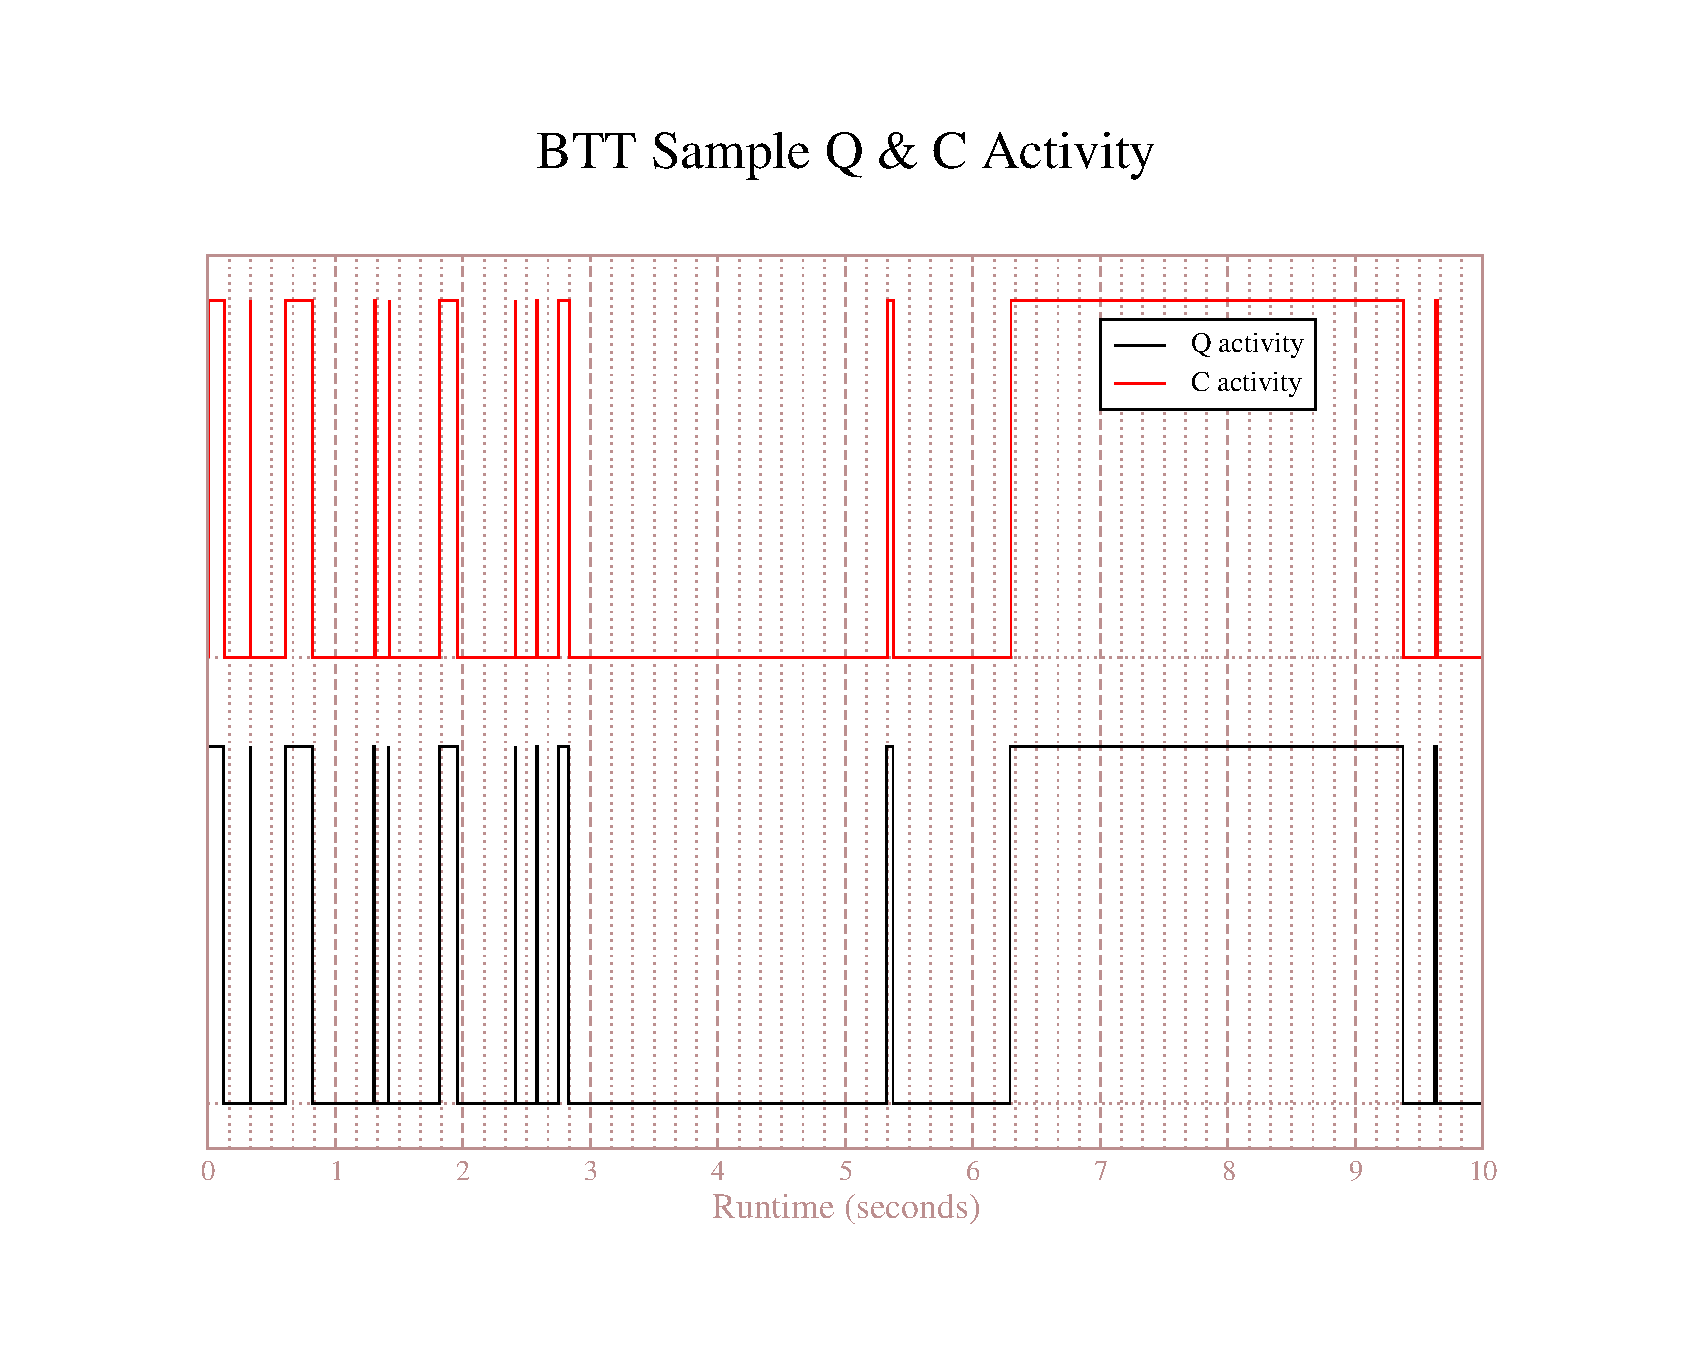
\epsfig{file=activity.eps,width=4.5in}
  \caption{\label{fig:activity}Simple Activity Chart}
  \end{figure}

  When the black line (system Q activity) is \emph{high}, then the system
  is seeing relatively continuous incoming queues. Conversely, when it is
  low, it represents an extended period of time where no queue requests
  were coming in. Similarly for the red line and C activity.

\newpage\section{\label{sec:hist}Histogram Data Files}

  The histogram data files provide information concerning incoming and
  outgoing IO sizes (in blocks). For simplicity, the histogram buckets
  are one-for-one for sizes up to 1,024 blocks in the IO, and then a
  single bucket for all sizes greater than or equal to 1,024 blocks.

  The files are again in grace-friendly format, with the first set
  containing data for the first 1,023 buckets, and a separate set
  representing sizes $\ge 1024$ blocks. (This is done so that one can
  easily use a separate formatting specification for the latter set.)

  The first column (X values) is the various IO sizes, and the second
  column (Y values) represents the number of IOs of that size.

\subsection{\label{sec:qhist}Q Histogram Data File}

  Figure~\ref{fig:qhist} is a sample graph generated from data used during
  some real-world analysis\footnote{Note the logarithmic nature of the
  Y axis for this chart.}. With the visual representation provided by
  this, one can quickly discern some different characteristics between
  the 3 runs -- in particular, one can see that there is only a single
  red point (representing 8 blocks per IO), whereas the other two had
  multiple data points greater than 8 blocks.

  \begin{figure}[hb]
  \leavevmode\centering
  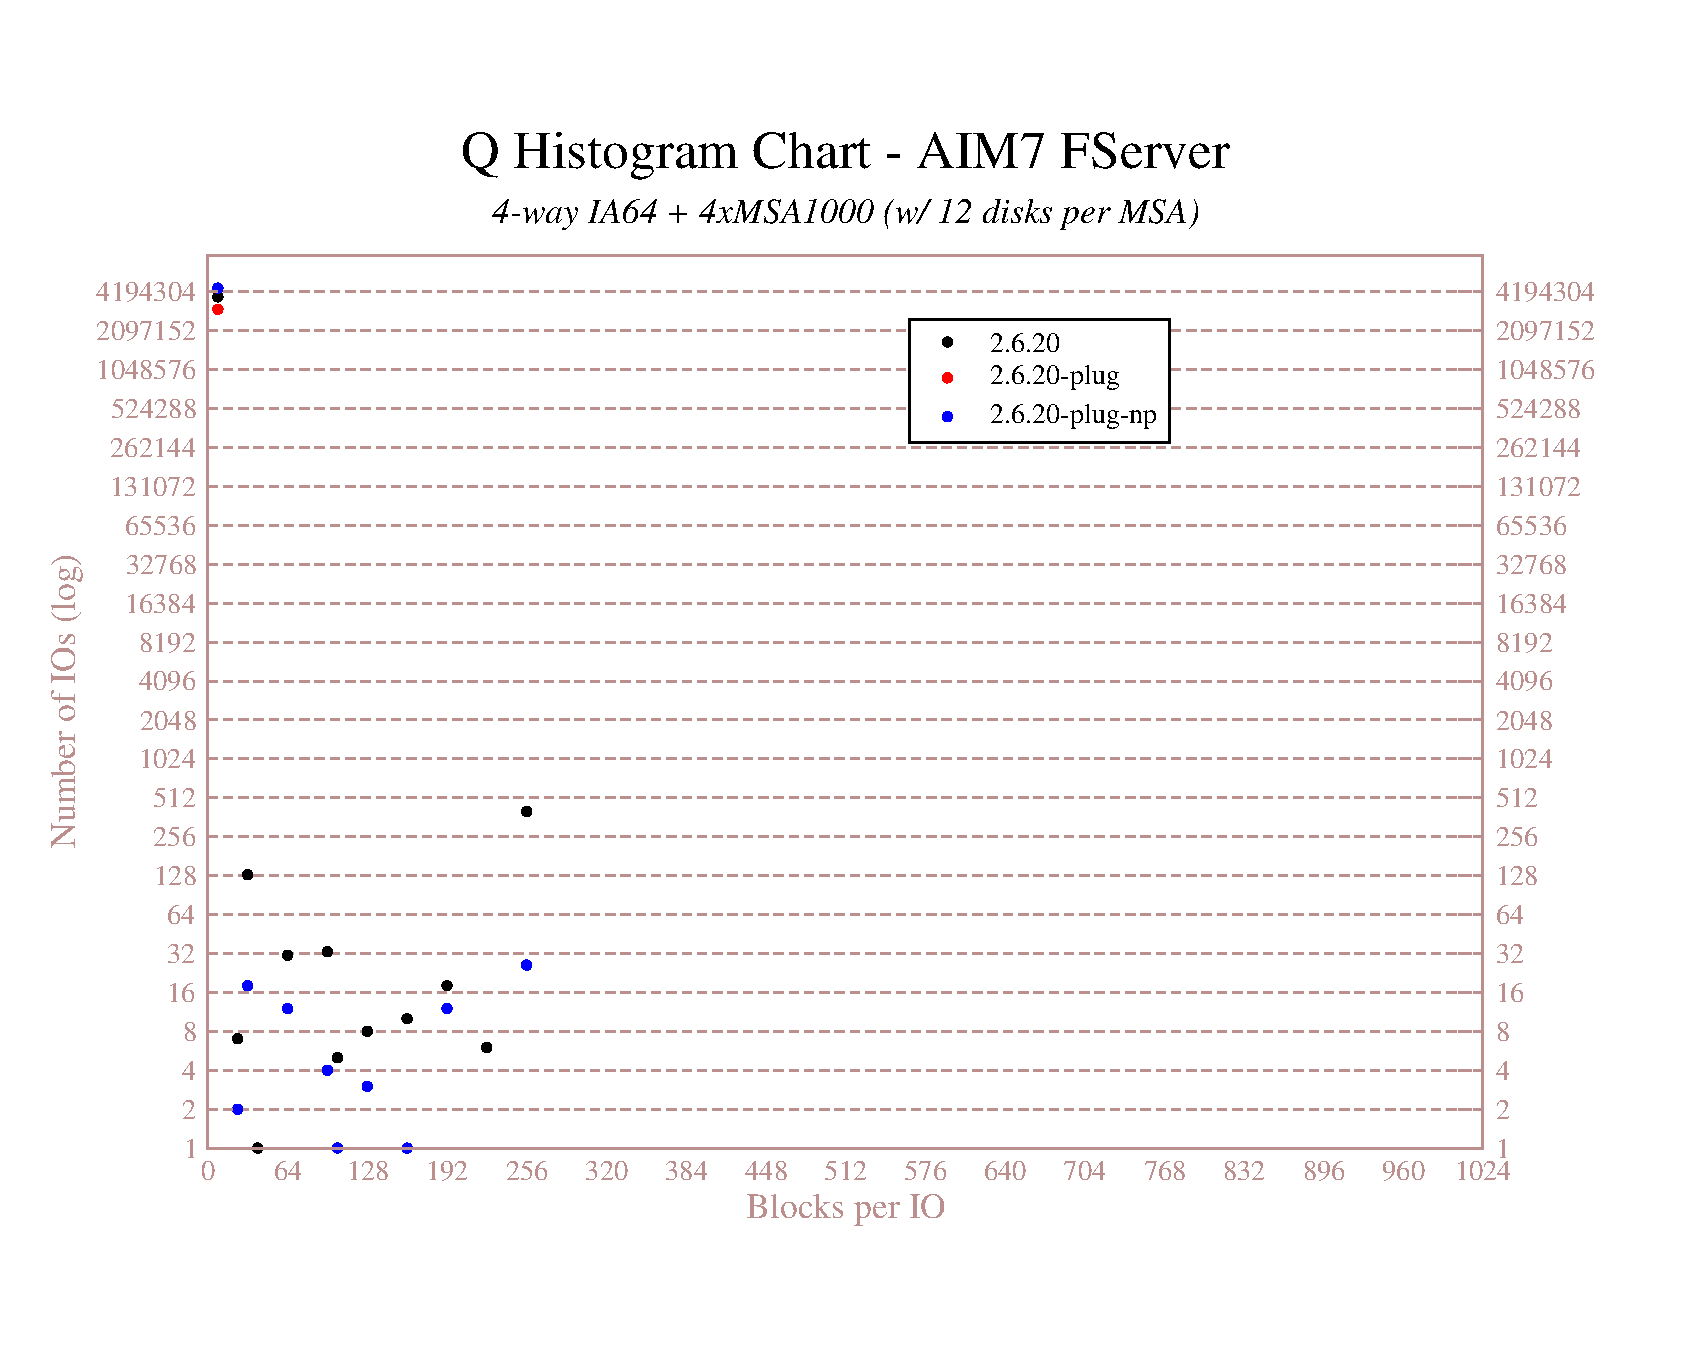
\epsfig{file=qhist.eps,width=4.5in}
  \caption{\label{fig:qhist}Q Histogram}
  \end{figure}

\subsection{\label{sec:dhist}D Histogram Data File}

  Figure~\ref{fig:dhist} is a sample graph generated from data used during
  some real-world analysis\footnote{Note the logarithmic nature of the
  Y axis for this chart.}. Again, visually, one can see that the black
  and blue dots are somewhat similar below about 192 blocks per IO going
  out. And then one can make the broad generalization of higher reds,
  lower blues and blacks in the middle.

  \begin{figure}[hb]
  \leavevmode\centering
  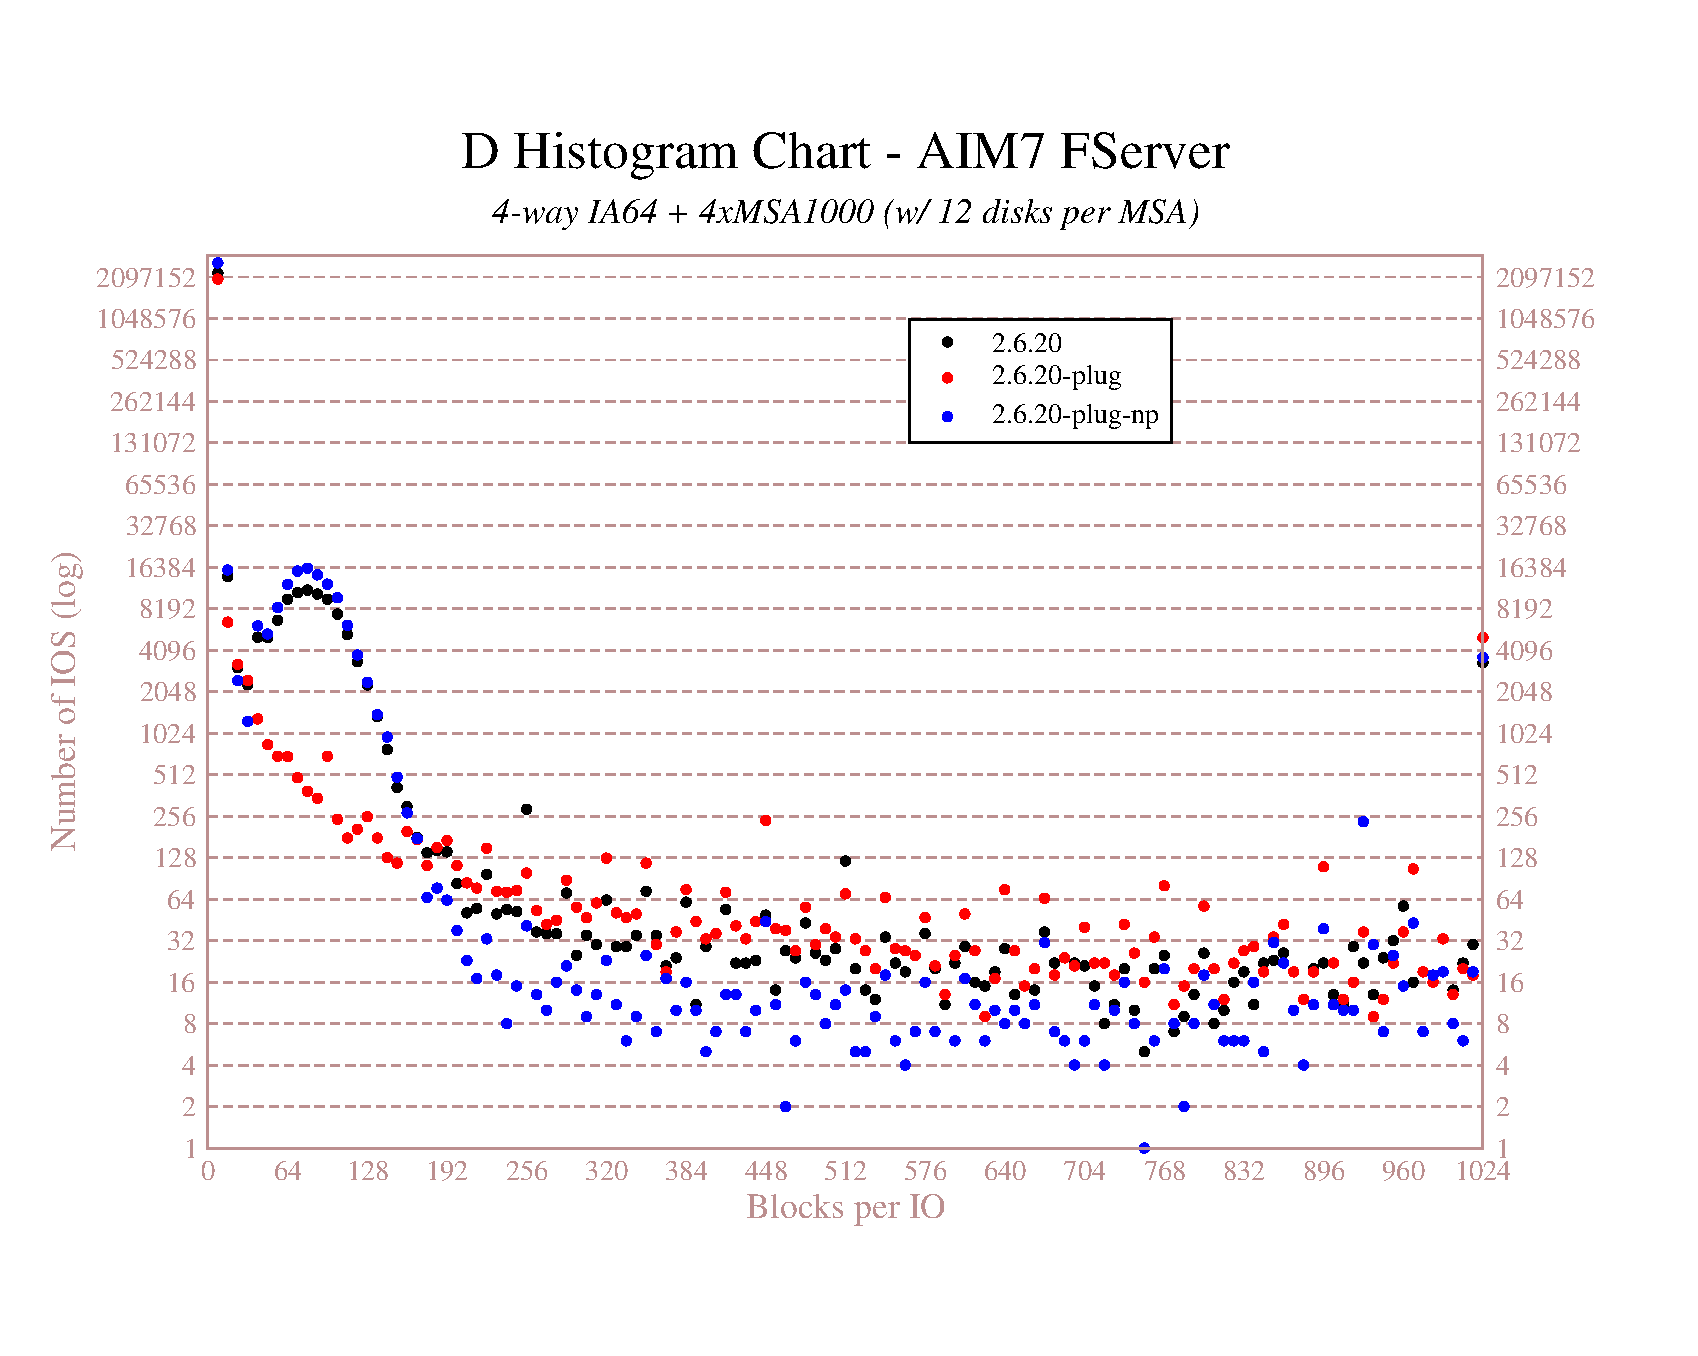
\epsfig{file=dhist.eps,width=4.5in}
  \caption{\label{fig:dhist}D Histogram}
  \end{figure}

\newpage\section{\label{sec:iostat}iostat Data File}
  \texttt{btt} attempts to produce the results from running an
  \texttt{iostat -x} command in parallel with the system as it is being
  traced. The fields (columns) generated by the \texttt{--iostat} or
  \texttt{-I} option can be seen from the following output snippet --
  note that the line has been split to fit on the printed page:

\begin{verbatim}
Device:       rrqm/s   wrqm/s     r/s     w/s    rsec/s    wsec/s
             rkB/s     wkB/s avgrq-sz avgqu-sz   await   svctm  %util   Stamp
...
(  8, 16)       0.00     0.00    0.00 1005.30      0.00 152806.36      
              0.00  76403.18   152.00    31.00    0.00    0.00   0.00   71.79
...
(  8, 16)       1.02     5.80    0.34    1.07      4.03     55.62
              2.02     27.81    42.13     0.61    0.00   21.90   0.00   TOTAL
\end{verbatim}

  Note that the STAMP field contains the runtime (in seconds) for that
  line of data.

\newpage\section{\label{sec:per-io}Per-IO Data File}

  \texttt{btt} can produce a text file containing time line data for each
  IO processed. The time line data contains rudimentary information for
  the following stages:

  \begin{itemize}
    \item queue traces
    \item get request traces
    \item insert traces
    \item merge traces
    \item issue traces
    \item completion traces
    \item remap traces
  \end{itemize}

  The \emph{--per-io-dump} or \emph{-p} option triggers this behavior,
  and will produce a file containing streams of IOs (separated by blank
  spaces), here is an example:

\begin{verbatim}
   20.002179731   8,32  Q         34+8
   20.002181199   8,32  I         34+8
   20.098329567   8,32  D         34+16
   20.002182760   8,32  Q         42+8
   20.002183613   8,32  M         42+8
   20.098329567   8,32  D         34+16
   20.692643206   8,32  C         34+16
\end{verbatim}

  The columns provide the following information:

  \begin{enumerate}
    \item Time of the trace (seconds from the start of the run)

    \item Device major/minor.

    \item Trace type 

    \item start block + number of blocks
  \end{enumerate}
  
  For this pair of initial IOs (Q traces at 20.002179731 and
  20.002182760), we can follow the insert and merge traces (20.002181199
  and 20.002183613 respectively), and the issue (duplicate entries for
  20.098329567), and the completion at 20.692643206. Every Q has its
  corresponding issue trace bounding any insert or merge operations.

\newpage\section{\label{sec:lat}\label{sec:lat-q2c}\label{sec:lat-d2c}Latency Data Files}

  The latency data files which can be optionally produced by \texttt{btt}
  provide per-IO latency information, one for total IO time (Q2C) and
  one for latencies induced by lower layer drivers and devices (D2C).

  In both cases, the first column (X values) represent runtime (seconds),
  while the second column (Y values) shows the actual latency for a
  command at that time (either Q2C or D2C).

\newpage\section{\label{sec:seek}Seek Data File}

  \texttt{btt} can also produce a data file containing all IO-to-IO sector
  deltas, providing seek information which can then be plotted. The
  produced data file contains 3 sets of data:

  \begin{enumerate}
     \item Combined data -- all read and write IOs

     \item Read data -- just seek deltas for reads

     \item Write data -- just seek deltas for writes
  \end{enumerate}

  The format of the data is to have the runtime values (seconds since
  the start of the run) in column 1 (X values); and the difference in
  sectors from the previous IO in column 2 (Y values). Here is a snippet
  of the first few items from a file:

\begin{verbatim}
# Combined
     0.000034733           35283790.0
     0.000106453           35283790.0
     0.005239009           35283950.0
     0.006968575           35283886.0
     0.007218709           35283694.0
     0.012145393           35283566.0
     0.014980835          -35848914.0
     0.024239323          -35848914.0
     0.024249402          -35848914.0
     0.025707095          -35849072.0
     ...
\end{verbatim}

  Figure~\ref{fig:seek} shows a simple graph that can be produced which
  provides visual details concerning seek patterns.

  \begin{figure}[h!]
  \leavevmode\centering
  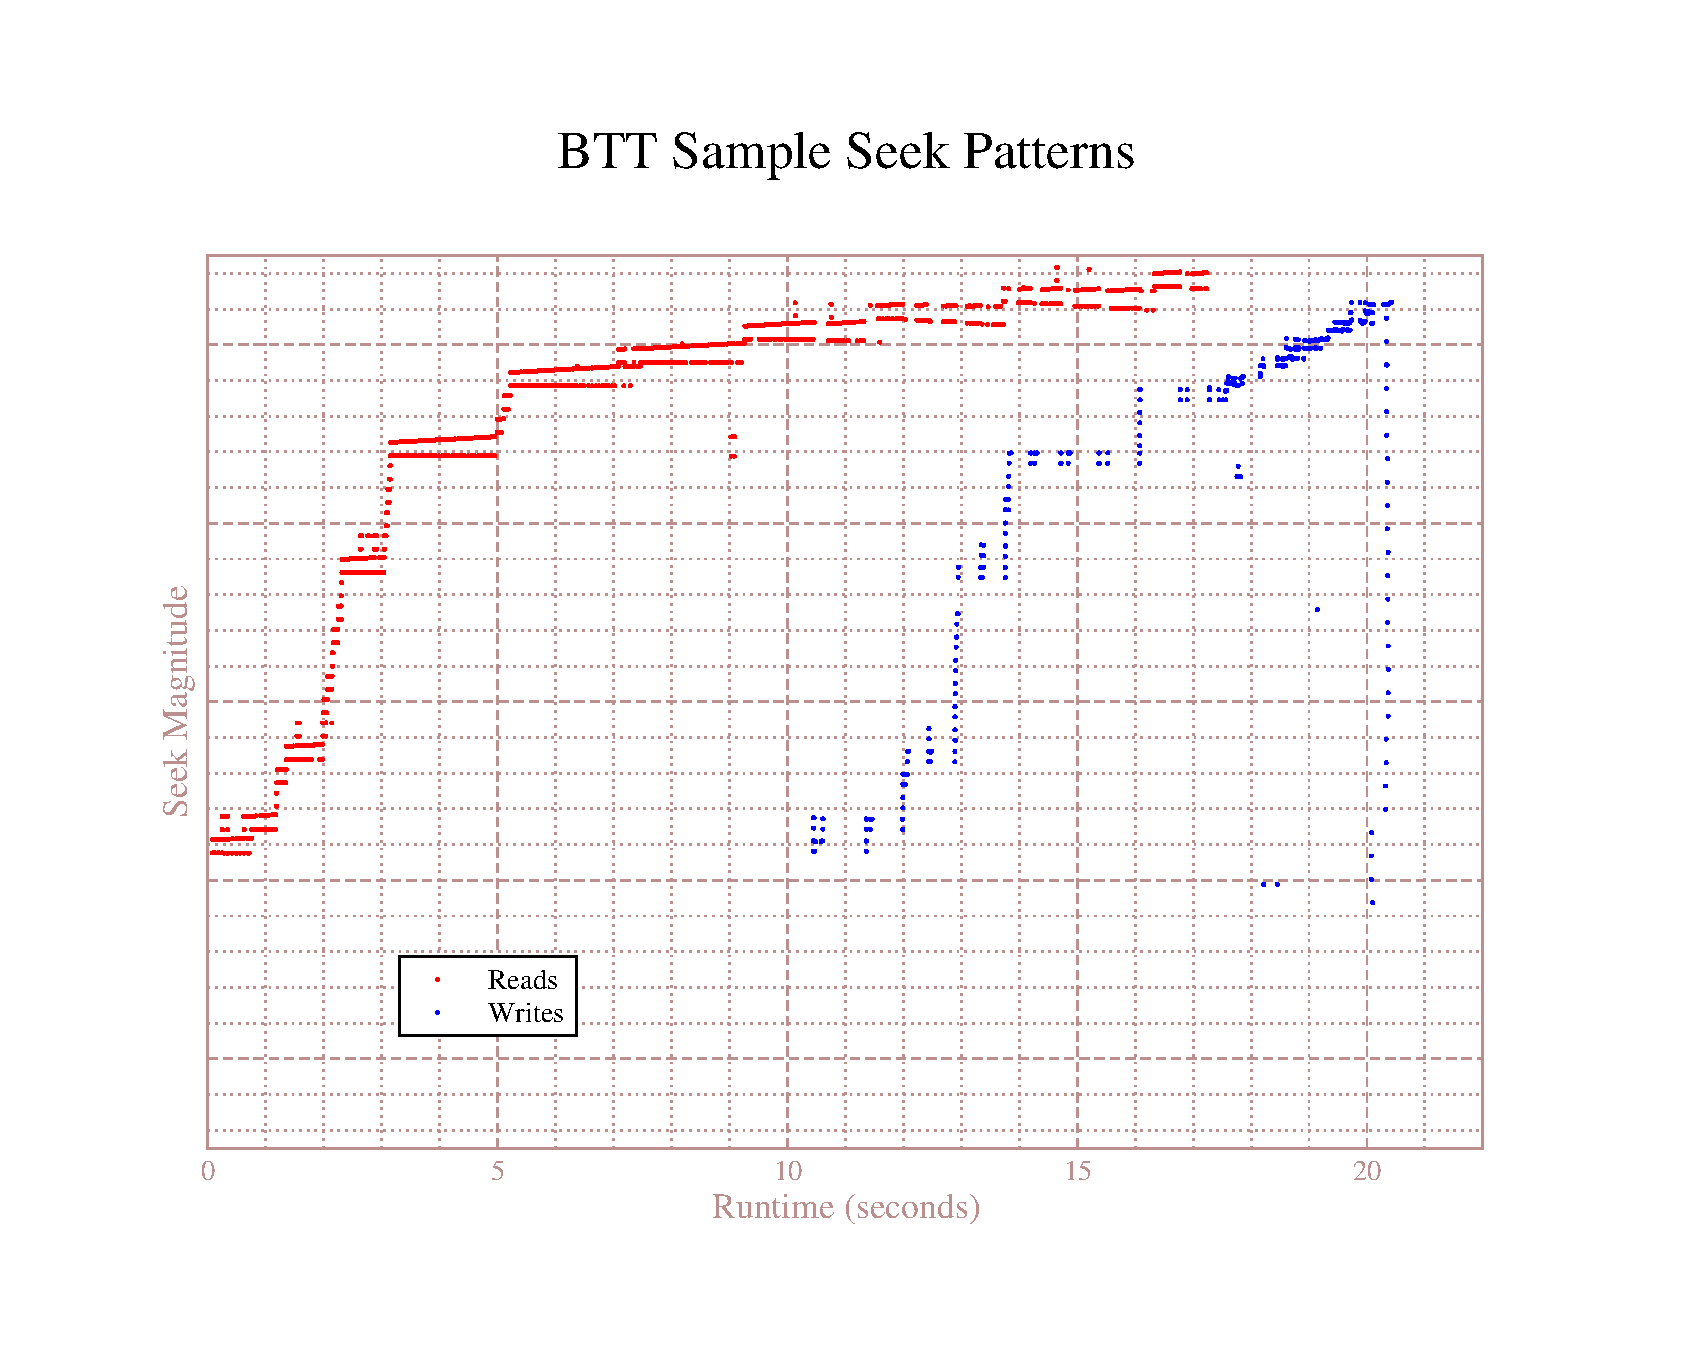
\epsfig{file=seek.eps,width=4.5in}
  \caption{\label{fig:seek}Seek Chart}
  \end{figure}
  \FloatBarrier

  The seek difference is calculated in one of two ways:

  \begin{description}
    \item[default] By default, the seek distance is calculated as the
    \emph{closest} distance between the previous IO and this IO. The
    concept of \emph{closeness} means that it could either be the
    \emph{end} of the previous IO and the beginning of the next, or the
    end of this IO and the start of the next.

    \item[\texttt{-a}] If the \texttt{-a} or \texttt{--seek-absolute}
    option is specified, then the seek distance is simply the difference
    between the end of the previous IO and the start of this IO.
  \end{description}

\newpage\section{\label{sec:cmd-line}Command Line}

\begin{verbatim}
Usage: \texttt{btt} 0.99.1 
[ -a               | --seek-absolute ]
[ -A               | --all-data ]
[ -B <output name> | --dump-blocknos=<output name> ]
[ -d <seconds>     | --range-delta=<seconds> ]
[ -D <dev;...>     | --devices=<dev;...> ]
[ -e <exe,...>     | --exes=<exe,...>  ]
[ -h               | --help ]
[ -i <input name>  | --input-file=<input name> ]
[ -I <output name> | --iostat=<output name> ]
[ -l <output name> | --d2c-latencies=<output name> ]
[ -M <dev map>     | --dev-maps=<dev map>
[ -o <output name> | --output-file=<output name> ]
[ -p <output name> | --per-io-dump=<output name> ]
[ -q <output name> | --q2c-latencies=<output name> ]
[ -s <output name> | --seeks=<output name> ]
[ -S <interval>    | --iostat-interval=<interval> ]
[ -t <sec>         | --time-start=<sec> ]
[ -T <sec>         | --time-end=<sec> ]
[ -V               | --version ]
[ -v               | --verbose ]
\end{verbatim}

\subsection{\label{sec:o-a}\texttt{--seek-absolute}/\texttt{-a}}

  When specified on the command line, this directs btt to calculate
  seek distances based solely upon the ending block address of one IO,
  and the start of the next.  By default \texttt{btt} uses the concept
  of the closeness to either the beginning or end of the previous IO. See
  section~\ref{sec:seek} for more details about seek distances.

\subsection{\label{sec:o-A}\texttt{--all-data}/\texttt{-A}}

  Normally \texttt{btt} will not print out verbose information
  concerning per-process and per-device data (as outlined in
  section~\ref{sec:detailed-data}). If you desire that level of 
  detail you can specify this option.

\subsection{\label{sec:o-B}\texttt{--dump-blocknos}/\texttt{-B}}

  This option will output absolute block numbers to three files prefixed
  by the specified output name:

  \begin{description}
    \item[\emph{prefix}\_\emph{device}\_r.dat] All read block numbers are
    output, first column is time (seconds), second is the block number,
    and the third column is the ending block number.

    \item[\emph{prefix}\_\emph{device}\_w.dat] All write block numbers are
    output, first column is time (seconds), second is the block number,
    and the third column is the ending block number.

    \item[\emph{prefix}\_\emph{device}\_c.dat] All block numbers (read
    and write) are output, first column is time (seconds), second is
    the block number, and the third column is the ending block number.
  \end{description}

\subsection{\label{sec:o-d}\texttt{--range-delta}/\texttt{-d}}

  Section~\ref{sec:activity} discussed how \texttt{btt} outputs a file
  containing Q and C activity, the notion of \emph{active} traces simply
  means that there are Q or C traces occurring within a certain period
  of each other. The default values is 0.1 seconds; with this option
  allowing one to change that granularity. The smaller the value, the
  more data points provided.

\subsection{\label{sec:o-D}\texttt{--devices}/\texttt{-D}}

  Normally, \texttt{btt} will produce data for all devices detected in
  the traces parsed. With this option, one can reduce the analysis to
  one or more devices provided in the string passed to this option. The
  device identifiers are the major and minor number of each device, and
  each device identifier is separated by a colon (:). A valid specifier
  for devices 8,0 and 8,8 would then be: \texttt{"8,0:8,8"}.

\subsection{\label{sec:o-e}\texttt{--exes}/\texttt{-e}}

  Likewise, \texttt{btt} will produce data for all processes (executables)
  found in the traces. With this option, one can specify which processes
  you want displayed in the output. The format of the string passed is
  a list of executable \emph{names} separated by commas (,). An example
  would be \texttt{"-e mkfs.ext3,mount"}.

\subsection{\label{sec:o-h}\texttt{--help}/\texttt{-h}}

  Prints out the simple help information, as seen at the top of
  section~\ref{sec:cmd-line}.

\subsection{\label{sec:o-i}\texttt{--input-file}/\texttt{-i}}

  Specifies the binary input file that \texttt{btt} will interpret traces
  in. See section~\ref{sec:getting-started} for information concerning
  binary trace files.

\subsection{\label{sec:o-I}\texttt{--iostat}/\texttt{-I}}

  This option triggers \texttt{btt} to generate iostat-like output to the
  file specified. Refer to section~\ref{sec:iostat} for more information
  on the output produced.

\subsection{\label{sec:o-l}\texttt{--d2c-latencies}/\texttt{-l}}

  This option instructs \texttt{btt} to generate the D2C latency file
  discussed in section~\ref{sec:lat-d2c}.

\subsection{\label{sec:o-M}\texttt{--dev-maps}/\texttt{-M}}

  Internal option, still under construction.

\subsection{\label{sec:o-o}\texttt{--output-file}/\texttt{-o}}

  Normally \texttt{btt} sends the statistical output (covered in
  section~\ref{sec:output-overview}) to standard out, if you specify
  this option this data is redirected to the file specified.

\subsection{\label{sec:o-p}\texttt{--per-io-dump}/\texttt{-p}}

  This option tells \texttt{btt} to generate the per IO dump file as
  discussed in section~\ref{sec:per-io}.

\subsection{\label{sec:o-q}\texttt{--q2c-latencies}/\texttt{-q}}

  This option instructs \texttt{btt} to generate the Q2C latency file
  discussed in section~\ref{sec:lat-q2c}.

\subsection{\label{sec:o-s}\texttt{--seeks}/\texttt{-s}}

  This option instruct \texttt{btt} to generate the seek data file
  discussed in section~\ref{sec:seek}.

\subsection{\label{sec:o-S}\texttt{--iostat-interval}/\texttt{-S}}

  The normal \texttt{iostat} command allows one to specify the snapshot
  interval, likewise, \texttt{btt} allows one to specify how many seconds
  between its generation of snapshots of the data via this option. Details
  about the iostat-like capabilities of \texttt{btt} may be found in
  section~\ref{sec:iostat}.

\subsection{\label{sec:o-tT}\texttt{--time-start}/\texttt{-t} and
\texttt{--time-end}/\texttt{T}}

  \begin{quote}
    \emph{This \texttt{btt} capability is still under construction, results are
    not always consistent at this point in time.}
  \end{quote}

  These options allow one to dictate to \texttt{btt} when to start and stop
  parsing of trace data in terms of seconds since the start of the run. The
  trace chosen will be between the start time (or 0.0 if not
  specified) and end time (or the end of the run) specified. 

\subsection{\label{sec:o-V}\texttt{--version}/\texttt{-V}}

  Prints out the \texttt{btt} version, and exits.

\subsection{\label{sec:o-v}\texttt{--verbose}/\texttt{-v}}

  While \texttt{btt} is processing data, it will put out periodic (1-second
  granularity) values describing the progress it is making through the
  input trace stream. The value describes how many traces have been
  processed. At the end of the run, the overall number of traces, trace
  rate (number of thousands of traces per second), and the real time for
  trace processing and output are displayed. Example (note: the interim
  trace counts are put out with carriage returns, hence, they overwrite
  each time):

\begin{verbatim}
# btt -i bp.bin -o btt -v
Sending range data to bttX.dat
Sending stats data to bttX.avg
 287857 t
1414173 t
1691581 t
...
4581291 traces @ 279.7 Ktps
16.379036+0.000005=16.379041
\end{verbatim}

\newpage\section{\label{sec:appendix}Appendix: Sample \texttt{btt}
Output}
  
  Here is a complete output file from a btt run, illustrating a lot of the
  capabilities of btt.

\begin{verbatim}
==================== All Devices ====================

            ALL           MIN           AVG           MAX           N
--------------- ------------- ------------- ------------- -----------
Q2Q               0.000000001   0.000015439   0.067431982     4485897
Q2I               0.000000277   0.000005085  12.844603081     4485736
I2D               0.000000869   0.000721745  12.845117057     4485736
D2C               0.000151807   0.005254051   0.097569048     4485736
Q2C               0.000156268   0.005980882  12.864868116     4485736

\end{verbatim}
\newpage\begin{verbatim}

==================== Device Overhead ====================

       DEV |    Q2I    I2D    D2C
---------- | ------ ------ ------
 (  8,160) |   0.0%   1.6%  98.4%
 (  8,176) |   0.1%  20.0%  79.9%
 (  8,208) |   1.2%  69.2%  29.5%
 ( 65, 32) |   0.0%   1.1%  98.8%
 ( 65, 64) |   0.0%   3.6%  96.4%
 ( 65,176) |   0.0%   2.5%  97.4%
 ( 65, 96) |   0.0%  15.3%  84.6%
 (  8,224) |   0.0%   1.7%  98.3%
 ( 65,112) |   0.0%   2.4%  97.6%
 (  8,240) |   0.0%   2.3%  97.7%
 ( 65,192) |   0.0%  19.4%  80.6%
 ( 65,240) |   0.0%   1.3%  98.7%
 ( 65, 48) |   0.0%   2.3%  97.7%
 (  8, 32) |   0.0%   7.0%  93.0%
 ( 66, 80) |   0.1%   9.9%  90.0%
 ( 66, 32) |   0.0%   0.7%  99.3%
 ( 65,224) |   0.0%  18.1%  81.9%
 ( 65,144) |   0.1%  39.5%  60.5%
 (  8,144) |   0.0%   0.7%  99.3%
 ( 66,144) |   0.0%   1.5%  98.5%
 ( 66,128) |   0.0%   3.0%  97.0%
 ( 66,176) |   0.0%  12.5%  87.4%
 ( 66,224) |   0.0%  10.2%  89.8%
 ( 66,192) |   0.0%   2.1%  97.9%
 ( 66,160) |   0.0%   9.4%  90.5%
 ( 66,240) |   0.0%   9.8%  90.2%
 ( 66,112) |   0.1%  24.2%  75.7%
 (  8, 64) |   0.0%   9.6%  90.4%
 ( 65,160) |   0.2%  26.2%  73.7%
 ( 65,208) |   0.0%   2.0%  98.0%
 ( 66, 16) |   0.0%   4.5%  95.5%
 ( 65,  0) |   0.0%   2.2%  97.8%
 ( 65, 16) |   0.0%   1.8%  98.1%
 ( 66,208) |   0.0%   2.7%  97.3%
 (  8,128) |   0.2%  23.7%  76.1%
 ( 65, 80) |   0.0%  20.0%  80.0%
 (  8,112) |   0.0%   1.2%  98.7%
 ( 65,128) |   0.0%   1.9%  98.1%
 ( 66, 64) |   0.0%  12.1%  87.9%
 ( 66,  0) |   0.0%   7.2%  92.8%
 ( 66, 48) |   0.0%   2.6%  97.4%
 (  8,192) |   0.0%   2.3%  97.7%
 ( 67, 16) |   0.0%   0.8%  99.2%
 ( 66, 96) |   0.0%  12.3%  87.7%
 (  8, 96) |   0.0%  10.3%  89.7%
 (  8, 80) |   0.0%   1.7%  98.3%
 (  8, 48) |   0.0%   0.7%  99.2%
 ( 67,  0) |   0.0%   2.6%  97.4%

\end{verbatim}
\newpage\begin{verbatim}

==================== Device Merge Information ====================

       DEV |       #Q       #D   Ratio |   BLKmin   BLKavg   BLKmax    Total
---------- | -------- -------- ------- | -------- -------- -------- --------
 (  8,160) |    75145    47890     1.6 |        8       12     1024   601160
 (  8,176) |    91374    55492     1.6 |        8       13     1024   730992
 (  8,208) |   101039    63944     1.6 |        8       12     1024   809256
 ( 65, 32) |    67919    44494     1.5 |        8       12     1024   543352
 ( 65, 64) |   114614    77396     1.5 |        8       11     1024   916968
 ( 65,176) |    93808    62746     1.5 |        8       11     1024   750464
 ( 65, 96) |    95537    51705     1.8 |        8       14     1024   764296
 (  8,224) |    95435    49753     1.9 |        8       15     1024   765560
 ( 65,112) |   100020    63530     1.6 |        8       12     1024   800160
 (  8,240) |    72282    44700     1.6 |        8       12     1024   578256
 ( 65,192) |    95175    59010     1.6 |        8       12     1024   761400
 ( 65,240) |    86334    53548     1.6 |        8       12     1024   690984
 ( 65, 48) |    69623    44652     1.6 |        8       12     1024   556984
 (  8, 32) |    97816    63116     1.5 |        8       12     1024   782528
 ( 66, 80) |   110873    71526     1.6 |        8       12     1024   886984
 ( 66, 32) |    79242    53134     1.5 |        8       11     1024   633936
 ( 65,224) |   122788    66180     1.9 |        8       14     1024   982304
 ( 65,144) |   116636    70205     1.7 |        8       13     1024   933416
 (  8,144) |    72014    49047     1.5 |        8       11     1024   576112
 ( 66,144) |   109244    70613     1.5 |        8       12     1024   873952
 ( 66,128) |   104688    65381     1.6 |        8       12     1024   837504
 ( 66,176) |    79627    47894     1.7 |        8       13     1024   637016
 ( 66,224) |    88754    58159     1.5 |        8       12     1024   710032
 ( 66,192) |    88919    55417     1.6 |        8       12     1024   711464
 ( 66,160) |   102908    71156     1.4 |        8       11     1024   823264
 ( 66,240) |    94190    66472     1.4 |        8       11     1024   753520
 ( 66,112) |   138799    82027     1.7 |        8       13     1024  1110392
 (  8, 64) |   105011    63892     1.6 |        8       13     1024   840112
 ( 65,160) |    93383    55579     1.7 |        8       13     1024   747064
 ( 65,208) |   109771    67987     1.6 |        8       12     1024   878168
 ( 66, 16) |    96703    56613     1.7 |        8       13     1024   773624
 ( 65,  0) |    83752    51532     1.6 |        8       13     1024   670032
 ( 65, 16) |    64538    35982     1.8 |        8       14     1024   516320
 ( 66,208) |    90636    54306     1.7 |        8       13     1024   725088
 (  8,128) |    96202    59653     1.6 |        8       13     1024   776192
 ( 65, 80) |   107945    65672     1.6 |        8       13     1024   863704
 (  8,112) |    78235    52847     1.5 |        8       11     1024   625880
 ( 65,128) |   104631    63106     1.7 |        8       13     1024   837048
 ( 66, 64) |    86365    50956     1.7 |        8       13     1024   690920
 ( 66,  0) |    90413    46722     1.9 |        8       15     1024   723304
 ( 66, 48) |   106631    65219     1.6 |        8       13     1024   853048
 (  8,192) |    80591    47154     1.7 |        8       13     1024   644728
 ( 67, 16) |    72314    48487     1.5 |        8       11     1024   578512
 ( 66, 96) |    90990    54454     1.7 |        8       13     1024   727920
 (  8, 96) |   110805    73522     1.5 |        8       12     1024   886440
 (  8, 80) |    85032    56643     1.5 |        8       12     1024   680400
 (  8, 48) |    87374    57544     1.5 |        8       12     1024   698992
 ( 67,  0) |    79611    53515     1.5 |        8       11     1024   636888
---------- | -------- -------- ------- | -------- -------- -------- --------
       DEV |       #Q       #D   Ratio |   BLKmin   BLKavg   BLKmax    Total
     TOTAL |  4485736  2790572     1.6 |        8       12     1024 35896640

\end{verbatim}
\newpage\begin{verbatim}

==================== Device Seek Information ====================

       DEV |          NSEEKS            MEAN          MEDIAN | MODE           
---------- | --------------- --------------- --------------- | ---------------
 (  8,160) |           47890        203945.5               0 | 0(2496)
 (  8,176) |           55492        252948.8               0 | 0(2360)
 (  8,208) |           63944        167845.3               0 | 0(4327)
 ( 65, 32) |           44494        224708.3               0 | 0(2683)
 ( 65, 64) |           77396        197838.0               0 | 0(2532)
 ( 65,176) |           62746        168400.5               0 | 0(2675)
 ( 65, 96) |           51705        162500.2               0 | 0(2778)
 (  8,224) |           49753        206665.7               0 | 0(2753)
 ( 65,112) |           63530        146289.8               0 | 0(2598)
 (  8,240) |           44700        167258.3               0 | 0(2735)
 ( 65,192) |           59010        217004.7               0 | 0(2724)
 ( 65,240) |           53548        278194.8               0 | 0(2415)
 ( 65, 48) |           44652        180710.3               0 | 0(2660)
 (  8, 32) |           63116        234049.5               0 | 0(2473)
 ( 66, 80) |           71526        184981.9               0 | 0(2455)
 ( 66, 32) |           53134        198369.5               0 | 0(2415)
 ( 65,224) |           66180        157948.5               0 | 0(2859)
 ( 65,144) |           70205        195689.7               0 | 0(2734)
 (  8,144) |           49047        169282.7               0 | 0(2574)
 ( 66,144) |           70613        149265.7               0 | 0(2717)
 ( 66,128) |           65381        165931.1               0 | 0(2687)
 ( 66,176) |           47894        199744.8               0 | 0(3096)
 ( 66,224) |           58159        161603.9               0 | 0(2738)
 ( 66,192) |           55417        153055.3               0 | 0(2828)
 ( 66,160) |           71156        126479.4               0 | 0(2739)
 ( 66,240) |           66472        142014.0               0 | 0(2933)
 ( 66,112) |           82027        115471.3               0 | 0(2961)
 (  8, 64) |           63892        136632.0               0 | 0(2655)
 ( 65,160) |           55579        154668.3               0 | 0(3377)
 ( 65,208) |           67987        152829.1               0 | 0(2523)
 ( 66, 16) |           56613        150652.8               0 | 0(2886)
 ( 65,  0) |           51532        186889.7               0 | 0(2765)
 ( 65, 16) |           35982        327187.6               0 | 0(2756)
 ( 66,208) |           54306        243784.1               0 | 0(3076)
 (  8,128) |           59653        170797.2               0 | 0(2800)
 ( 65, 80) |           65672        224501.4               0 | 0(2452)
 (  8,112) |           52847        213100.3               0 | 0(2417)
 ( 65,128) |           63106        207821.8               0 | 0(2686)
 ( 66, 64) |           50956        198045.0               0 | 0(2896)
 ( 66,  0) |           46722        205476.3               0 | 0(3159)
 ( 66, 48) |           65219        142716.6               0 | 0(2869)
 (  8,192) |           47154        248778.6               0 | 0(2584)
 ( 67, 16) |           48487        193335.5               0 | 0(2879)
 ( 66, 96) |           54454        185100.7               0 | 0(2158)
 (  8, 96) |           73522        216187.1               0 | 0(2476)
 (  8, 80) |           56643        172561.8               0 | 0(2612)
 (  8, 48) |           57544        219104.1               0 | 0(2472)
 ( 67,  0) |           53515        161613.8               0 | 0(2990)
---------- | --------------- --------------- --------------- | ---------------
   Overall |          NSEEKS            MEAN          MEDIAN | MODE           
   Average |         2790572        185170.0               0 | 0(131433)

\end{verbatim}
\newpage\begin{verbatim}
==================== Plug Information ====================

       DEV |    # Plugs # Timer Us  | % Time Q Plugged
---------- | ---------- ----------  | ----------------
 (  8,160) |      45092(         0) |   0.003021834%
 (  8,176) |      49430(         0) |   0.003724997%
 (  8,208) |      58950(         0) |   0.004506453%
 ( 65, 32) |      41617(         0) |   0.002710008%
 ( 65, 64) |      74294(         0) |   0.004971739%
 ( 65,176) |      59764(         0) |   0.003827258%
 ( 65, 96) |      47495(         0) |   0.004012641%
 (  8,224) |      46806(         0) |   0.003724031%
 ( 65,112) |      60539(         0) |   0.004272802%
 (  8,240) |      41797(         0) |   0.002832794%
 ( 65,192) |      54754(         0) |   0.004049758%
 ( 65,240) |      50757(         0) |   0.003466684%
 ( 65, 48) |      41749(         0) |   0.002783118%
 (  8, 32) |      59486(         0) |   0.004102902%
 ( 66, 80) |      67519(         0) |   0.004698104%
 ( 66, 32) |      50441(         0) |   0.003229586%
 ( 65,224) |      60219(         0) |   0.005114778%
 ( 65,144) |      64699(         0) |   0.005185315%
 (  8,144) |      46237(         0) |   0.002824578%
 ( 66,144) |      67605(         0) |   0.004459997%
 ( 66,128) |      62418(         0) |   0.004598612%
 ( 66,176) |      43007(         0) |   0.003277143%
 ( 66,224) |      54724(         0) |   0.003682546%
 ( 66,192) |      52395(         0) |   0.003611178%
 ( 66,160) |      67775(         0) |   0.004347445%
 ( 66,240) |      62892(         0) |   0.003906526%
 ( 66,112) |      72351(         0) |   0.005906198%
 (  8, 64) |      59642(         0) |   0.004275726%
 ( 65,160) |      50303(         0) |   0.003841735%
 ( 65,208) |      64750(         0) |   0.004655374%
 ( 66, 16) |      53443(         0) |   0.003936557%
 ( 65,  0) |      48450(         0) |   0.003301599%
 ( 65, 16) |      33047(         0) |   0.002447028%
 ( 66,208) |      51060(         0) |   0.003674090%
 (  8,128) |      52664(         0) |   0.004009472%
 ( 65, 80) |      61974(         0) |   0.004623080%
 (  8,112) |      50106(         0) |   0.003284028%
 ( 65,128) |      60047(         0) |   0.004267589%
 ( 66, 64) |      47590(         0) |   0.003646022%
 ( 66,  0) |      43413(         0) |   0.003600655%
 ( 66, 48) |      61984(         0) |   0.004440717%
 (  8,192) |      44294(         0) |   0.003120507%
 ( 67, 16) |      45482(         0) |   0.002852274%
 ( 66, 96) |      50099(         0) |   0.003970858%
 (  8, 96) |      70266(         0) |   0.004743310%
 (  8, 80) |      53676(         0) |   0.003530690%
 (  8, 48) |      54672(         0) |   0.003527266%
 ( 67,  0) |      50418(         0) |   0.003217817%
---------- | ---------- ----------  | ----------------
       DEV |    # Plugs # Timer Us  | % Time Q Plugged
   OVERALL |      54420(         0) |   0.003871155%
\end{verbatim}
\end{document}
